\documentclass[tikz,border=2pt]{standalone}
\usepackage{lmodern}
\usetikzlibrary{arrows.meta,calc,backgrounds}
\definecolor{accent}{HTML}{365F7D}
\begin{document}
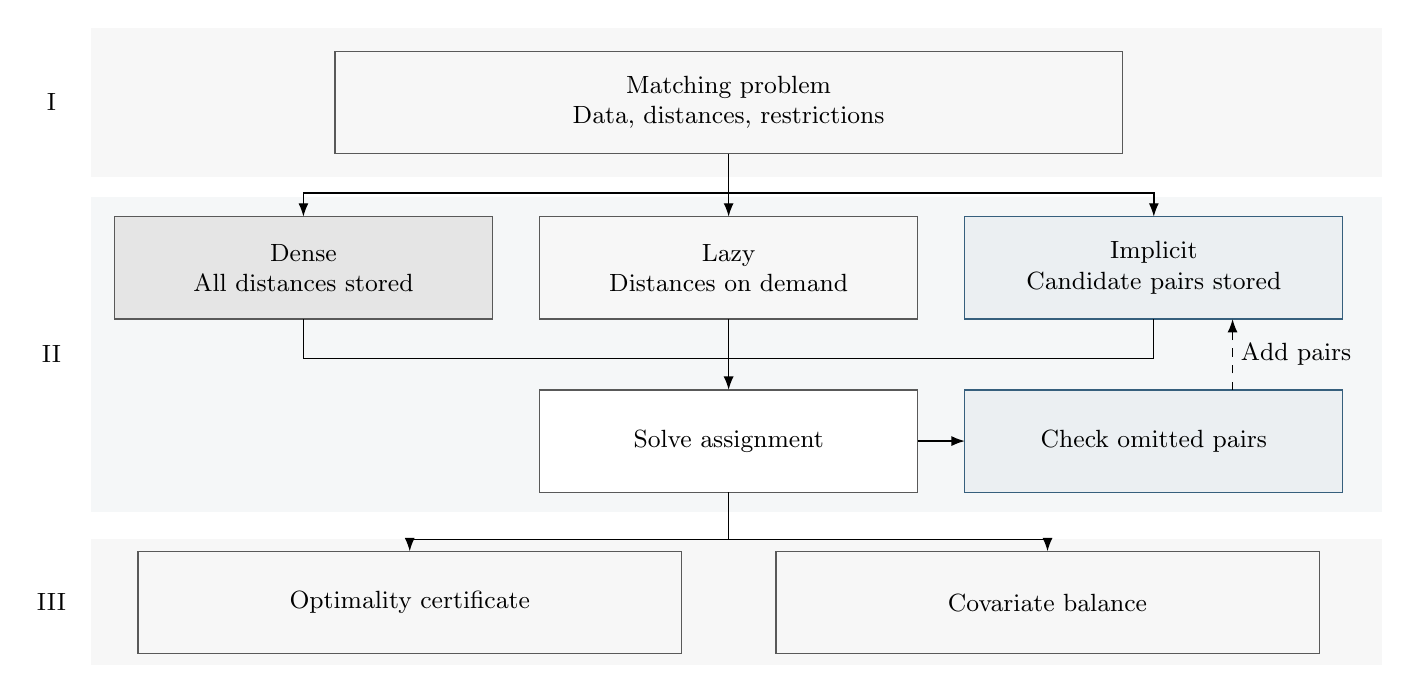
\begin{tikzpicture}[
  font=\fontsize{9}{11}\selectfont,text=black,
  box/.style={draw=black!65,fill=white,line width=.45pt,align=center,
    text width=42mm,minimum height=13mm,inner sep=3mm},
  arrow/.style={-{Latex[length=1.7mm]},line width=.5pt},
  every node/.style={outer sep=0pt}]
  \begin{scope}[on background layer]
    \fill[black!3] (-8.1,.95) rectangle (8.3,-.95);
    \fill[accent!5] (-8.1,-1.2) rectangle (8.3,-5.2);
    \fill[black!3] (-8.1,-5.55) rectangle (8.3,-7.15);
  \end{scope}
  \node at (-8.6,0) {I};
  \node at (-8.6,-3.2) {II};
  \node at (-8.6,-6.35) {III};
  \node[box,text width=94mm,fill=black!3] (data) at (0,0)
    {Matching problem\\
     Data, distances, restrictions};

  \node[box,fill=black!10] (dense) at (-5.4,-2.1)
    {Dense\\All distances stored};
  \node[box,fill=black!3] (lazy) at (0,-2.1)
    {Lazy\\Distances on demand};
  \node[box,draw=accent,fill=accent!10] (implicit) at (5.4,-2.1)
    {Implicit\\Candidate pairs stored};
  \coordinate (fork) at (0,-1.15);
  \draw (data.south) -- (fork);
  \draw[arrow] (fork) -| (dense.north);
  \draw[arrow] (fork) -- (lazy.north);
  \draw[arrow] (fork) -| (implicit.north);

  \node[box] (solve) at (0,-4.3)
    {Solve assignment};
  \coordinate (join) at (0,-3.25);
  \draw (dense.south) |- (join);
  \draw (implicit.south) |- (join);
  \draw[arrow] (lazy.south) -- (solve.north);

  \node[box,draw=accent,fill=accent!10] (check) at (5.4,-4.3)
    {Check omitted pairs};
  \draw[arrow] (solve.east) -- (check.west);
  \draw[arrow,dashed] ([xshift=10mm]check.north) --
    node[right,inner sep=3pt] {Add pairs}
    ([xshift=10mm]implicit.south);
  \node[box,text width=63mm,fill=black!3] (cert) at (-4.05,-6.35)
    {Optimality certificate};
  \node[box,text width=63mm,fill=black!3] (balance) at (4.05,-6.35)
    {Covariate balance};
  \coordinate (out) at (0,-5.55);
  \draw (solve.south) -- (out);
  \draw[arrow] (out) -| (cert.north);
  \draw[arrow] (out) -| (balance.north);
\end{tikzpicture}
\end{document}




